\documentclass{beamer}
\usepackage[utf8]{inputenc}
\usepackage{listings}
\usepackage{booktabs}
\usepackage{amssymb}
\usepackage{amsmath}
\usepackage{bm}
\usepackage{enumitem}
\usepackage{hyperref}
\usepackage{nicefrac}
\usepackage[export]{adjustbox}
\usepackage{svg}

\usetheme{Madrid}
\definecolor{mlpblue}{rgb}{0.1, 0.14, 0.24}

\useoutertheme{infolines} % Alternatively: miniframes, infolines, split
\useinnertheme{circles}
\usecolortheme[named=mlpblue]{structure}

\lstset{basicstyle=\footnotesize\ttfamily,breaklines=true}

%------------------------------------------------------------
%This block of code defines the information to appear in the
%Title page
\title[Contrastive Optimization]{Crossing Cross-Entropy:}

\subtitle{The Power of Provably Faithful Interpretability}

\author[Mathematical Foundations of DL] % optional
{J.~Setpal} 

\date{October 25, 2024}

% \titlegraphic{
\includegraphics[width=7cm]{../shared/logo-long.pdf}}

%End of title page configuration block
%------------------------------------------------------------

%The next block of commands puts the table of contents at the 
%beginning of each section and highlights the current section:

\AtBeginSection[]
{
  \begin{frame}
    \frametitle{Outline}
    \tableofcontents[currentsection]
  \end{frame}
}
% ------------------------------------------------------------


\begin{document}

\frame{\titlepage}

\begin{frame}{What is Interpretability?}
		\begin{columns}
		\begin{column}{0.5\textwidth}
			\begin{center}
				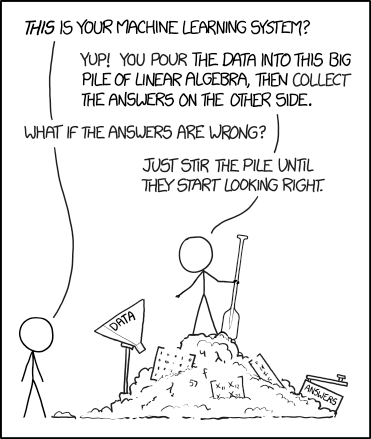
\includegraphics[width=5cm]{img/1838} \pause
			\end{center}
		\end{column}
		\begin{column}{0.5\textwidth}
			Interpretability within Machine Learning is the \textbf{degree} to which we can understand the \textbf{cause} of a decision, and use it to consistently \underline{predict the model's prediction}. \pause \newline \\

			Traditionally, interpretability \& performance is seen as a trade-off.\footnote{Dziugaite,~Ben-David,~Roy.~[Arxiv 2020]} \pause \newline \\

			Our work demonstrates a deep intersect between these two \textit{seemingly} orthogonal research foci.
		\end{column}
	\end{columns}
\end{frame}

\begin{frame}{Overarching Motivation}
	\textbf{Goal:} Constrain learning to interpretable ``sanity checks''.
	\vspace{-1em}
	\begin{center}
		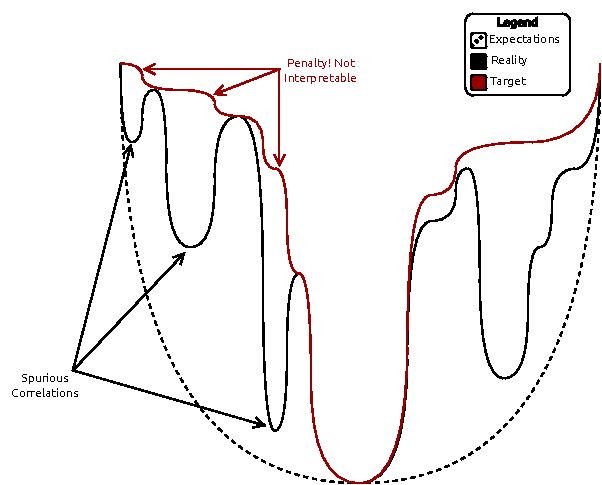
\includegraphics[width=.75\textwidth]{img/loss-landscape.pdf}
	\end{center}
\end{frame}

\begin{frame}{Contrastive Activation Maps ($\nicefrac{1}{2}$)}
	HiResCAMs are a \underline{provably faithful} interpretability technique:
	\begin{center}
		\vspace{-1em}
		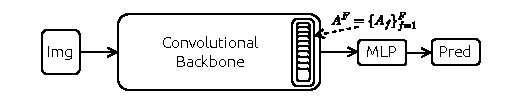
\includegraphics[width=\textwidth]{img/cams.pdf}
	\end{center}
	\vspace{-2em}
	\begin{gather}
		\tilde{\mathcal{A}}^{\text{HiResCAM}}_{c} = \sum^{F}_{f=1} \frac{\partial \hat{y}_c}{\partial A_f} \odot A_f
	\end{gather} \pause
	Provably faithful because:
	\vspace{-1em}
	\begin{gather}
		\hat{y}_c = \sum^{D_1, D_2}_{d_1, d_2} \tilde{\mathcal{A}}^{\text{HiResCAM}}_{c, d_1, d_2} + b_c
	\end{gather} \pause
	However, softmax-activated multi-class classification relies on \textbf{inter-class logit differences${}^{\bm{!!!}}$}, while HiResCAMs only re-construct \textit{absolute values}.
\end{frame}

\begin{frame}{Contrastive Activation Maps ($\nicefrac{2}{2}$)}
	To recover logit differences, we define \textbf{ContrastiveCAMs}:
	\begin{gather}
			\tilde{\mathcal{\bm{A}}}^{\text{contrastive}}_{(c_t, c_{t'})} := \left\{\tilde{\mathcal{\bm{A}}}_{c_t}^{\text{HiResCAM}} - \tilde{\mathcal{\bm{A}}}_{c_{t'}}^{\text{HiResCAM}}\right\}^{|c|-1}_{c_{t'} \in c \setminus c_t}
	\end{gather} \pause
	Next, we can now define an objective equivalent to cross-entropy:\footnote{with subtle changes to the architecture}
	\begin{gather}
		\max_{\theta} \sum^{D_1,D_2}_{d_1,d_2}\tilde{\mathcal{\bm{A}}}_{(c, c'),d_1,d_2}^{\text{contrastive}}\ \forall c' \in \mathbb{Z}_{+}(|c| - 1)
	\end{gather}
	\pause
	With one key difference: \textbf{we've preserved spatial information}.
\end{frame}

\begin{frame}{Understanding the Problem}
	We evaluated models trained using Cross-Entropy Loss using ContrastiveCAMs:

	\begin{center}
		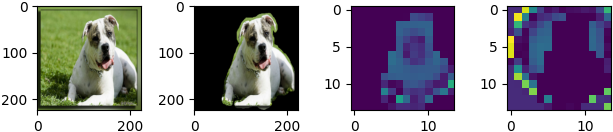
\includegraphics[width=\textwidth]{img/default.png}
	\end{center} \pause

	\textbf{Problem Statement:} For image classification tasks, Cross-Entropy motivates learning \textit{spurious correlations}. \pause \newline \\

	Provided the target class contains the largest logit, cross-entropy is happy. \pause \newline \\

	We can use ContrastiveCAMs to optimize our network under a ``foreground-only'' constraint!
\end{frame}

\begin{frame}{Contrastive Optimization}
	Cross-Entropy Loss is defined as follows:
	\begin{gather}
		\mathcal{J}(y, \hat{y}) = - \sum_{c \in C} y_c \log(\sigma_{\text{softmax}}(\hat{y}_c))
	\end{gather} \pause
	We derive cross-entropy as function of ContrastiveCAMs, then \textbf{penalize the background}:
	\begin{gather}
		\begin{split}
			&\mathcal{J}(\{\tilde{\mathcal{A}}_{c, i}^{\text{contrastive}}\}_i^{|c|}, h, c) = \\
			&-\log \left( \frac{1}{\sum_i \text{exp}\left({-\sum^{}h \odot \tilde{\mathcal{\bm{A}}}^{\text{contrastive}}_{(c, i)} + \sum |(1-h) \odot \tilde{\mathcal{\bm{A}}}^{\text{contrastive}}_{(c, i)}}|\right)} \right)
		\end{split}
	\end{gather} \pause
	The model learns to:
	\begin{enumerate}[label=\arabic*.]
		\item Use \textit{only} the foreground to base it's prediction.
		\item Treat the \textbf{background as noise}, and \underline{learn invariance to it}.
	\end{enumerate}
\end{frame}

\begin{frame}{Results (so far) ($\nicefrac{1}{2}$)}
	In-distribution fine-grained image classification on Oxford-IIIT Pets:
	\begin{table}[h]
		\centering
		\begin{tabular}{c|ccc}
			\toprule
			\textbf{Method}  & \textbf{Valid CE Loss}  & \textbf{Train Acc}   & \textbf{Valid Acc} \\
			\midrule
			Cross-Entropy & 3.605 & 5.1\% & 5.2\% \\
			Interpretable (Ours) & \bf 3.159 & \bf 96.9\% & \bf 51.5\% \\
			\bottomrule
		\end{tabular}
	\end{table} \pause
	Out-of-Distribution generalization performance on \href{https://www.kaggle.com/c/dogs-vs-cats}{Dogs v/s Cats dataset}:
	\begin{table}[h]
		\centering
		\begin{tabular}{c|c}
			\toprule
			\textbf{Method} & \textbf{Accuracy} \\
			\midrule
			Cross-Entropy & 77.0\% \\
			Interpretable (Ours) & \bf 83.4\% \\
			\bottomrule
		\end{tabular}
	\end{table}

\end{frame}

\begin{frame}{Results (so far) ($\nicefrac{2}{2}$)}
	\textbf{Before:}
	\begin{center}
		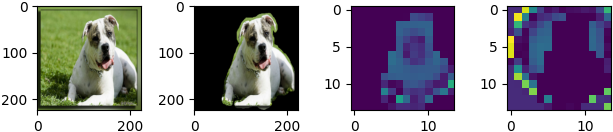
\includegraphics[width=\textwidth]{img/default.png}
	\end{center}

	\textbf{After:}
	\begin{center}
		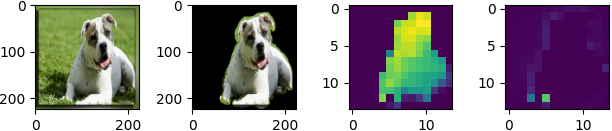
\includegraphics[width=\textwidth]{img/contrastive.png}
	\end{center}
\end{frame}

\begin{frame}{Next Steps}
	We're targeting the following next steps:
	\begin{enumerate}[label=\arabic*.]
		\item Exploring a level deeper: unpacking $\sum_{f=1}^F A_f$.
		\item Identifying the cause of the generalization gap in multiclass setting.
		\item Evaluating adversarial robustness.
		\item Mechanistic Interpretability study (circuit identification).
		\item Evaluating the approach at scale, using ImageNet-S.
	\end{enumerate}
	~\newline \pause
	\underline{Long-Term Objective:} Build proof-backed approaches to optimization that learn \textbf{intrinsically interpretable neural networks}.
\end{frame}

\begin{frame}{Thank you!}
	\begin{center}
		Have an awesome rest of your day!
	\end{center}
	\begin{center}
		\small
		\textbf{Slides:} \url{https://cs.purdue.edu/homes/jsetpal/slides/cont-opt.pdf} \\
		\textbf{Code:} \url{https://dagshub.com/jinensetpal/contrastive-optimization} \newline \\
		\textbf{Homepage:} \url{https://jinen.setpal.net/}
	\end{center}
\end{frame}

\end{document}
